%&pdflatex
\documentclass[11pt, a4paper]{article}
\usepackage{graphicx}
\usepackage{amsmath}
\usepackage{listings}
\usepackage{minted}
\usepackage{physics}
\usepackage{hyperref}
\hypersetup{
    colorlinks=true, %set true if you want colored links
    linktoc=all,     %set to all if you want both sections and subsections linked
    linkcolor=magenta,  %choose some color if you want links to stand out
}

\title{EE2703 Applied Programming Lab - Assignment No 8}
\author{
  \textbf{Name}: Abishek S\\
  \textbf{Roll Number}: EE18B001
}\date{\today}
\begin{document}
		
\maketitle 
\section{Abstract}
The goal of the assignment is the following :
\begin{itemize}
\item Obtaining the DFT of various functions using the fft module in numpy.
\item To analyse and correct the DFT obtained by plotting their spectrum.
\item To use DFT to estimate CTFT.
\end{itemize}
\usemintedstyle{manni}


\section{Assignment}
\subsection{Setting up the environment}
Importing the standard libraries
\begin{minted}[mathescape,escapeinside = ||]{python3}
#Importing Necessary Libraries 
from pylab import *
import sys
import matplotlib
\end{minted}


\subsection{EXAMPLE 1 - Introduction to FFT and IFFT}
{
To verify that the fft and the ifft are inverses of each other, we measure the error between the original function and the function predicted by taking ifft of fft of the original function.
}
\begin{minted}{python3}
x=rand(100)
X=fft(x)
y=ifft(X)
print(c_[x,y][:10])  #printing first 10 lines alone to get an idea 
			#of how close x and y values are
print('Maximum absolute error between x and y is :',abs(x-y).max())
\end{minted}
\begin{figure}[H]
   	\centering
   	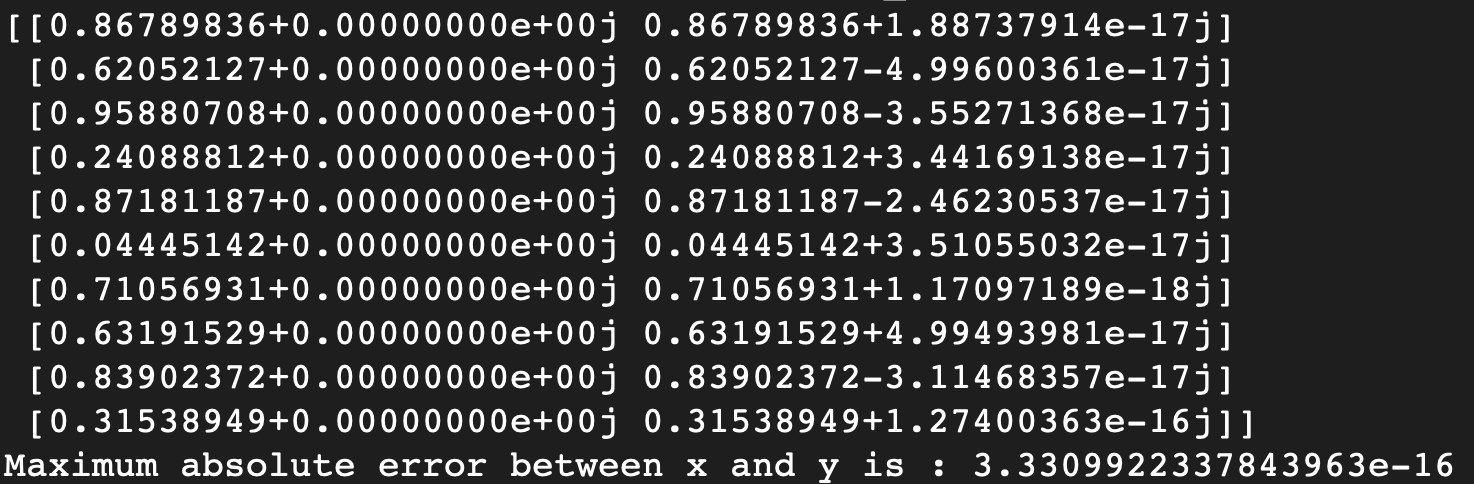
\includegraphics[scale=0.5]{ex1.png}
   	\label{fig:ex1}
   	\caption{Output of Example 1 Program}
\end{figure}
{
The smalll error is due to computer's numerical precision.
}

\subsection{EXAMPLE 2 - FFT of $\sin(5x)$, Trial 1}
{
We try to take the FFT of a sinusoid - $\sin(5t)$ to be precise.
\\We know that :
\[y = \sin(5t) = \frac{(e^{5jt}-e^{-5jt})}{2j}\]
\[Y(\omega) = \frac{1}{2j} [\delta(\omega-5) - \delta(\omega+5)]
\]
}
\begin{minted}{python3}
x=linspace(0,2*pi,128)
y=sin(10*x)
Y=fft(y)
figure()
subplot(2,1,1)
plot(abs(Y),lw=2)  #line width of 2
ylabel(r"$|Y|$",size=16)
title(r"Spectrum of $\sin(5t)$")
grid(True)  #for the grids to be shown
subplot(2,1,2)
plot(unwrap(angle(Y)),lw=2)
ylabel(r"Phase of $Y$",size=16)
xlabel(r"$k$",size=16)
grid(True)
savefig("ex2_i.png")  #Automatically saving the figure
show()
\end{minted}
\begin{figure}[H]
   	\centering
   	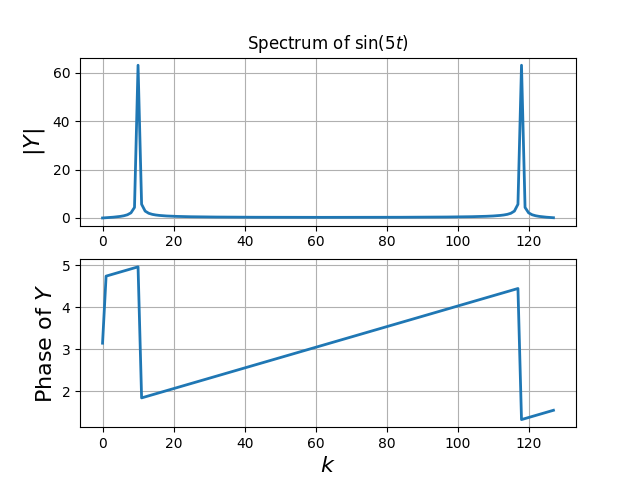
\includegraphics[scale=0.8]{ex2_i.png}
   	\label{fig:ex2_i}
   	\caption{Spectrum of $\sin(5t)$ - Trial 1}
\end{figure}
{
We get 2 peaks as expected but the peaks are in the wrong locations and the scale of the x axis is wrong. We also see that the height of peaks in the spectrum in wrong.
}


\subsection{EXAMPLE 2 - FFT of $\sin(5x)$, Trial 2} 
{
We correct the x axis by using w vector as the x axis. Then, we use fftshift() to correct the peaks' location by shifting the  $\pi$ to $2\pi$ to $-\pi$ to $0$ as it represents negative frequency. We also divide by the amplitude by number of samples to get the proper spectrum.
\\Finally, we also have to exclude the last sample as 0 and $2\pi$ represent the same frequency.
}
\begin{minted}{python3}
x=linspace(0,2*pi,129);x=x[:-1]  #last point is excluded
y=sin(5*x)
Y=fftshift(fft(y))/128.0  #fftshift converts from [0,2pi] to [-pi,pi] 
w=linspace(-64,63,128)
figure()
subplot(2,1,1)
plot(w,abs(Y),lw=2)
xlim([-10,10])
ylabel(r"$|Y|$",size=16)
title(r"Spectrum of $\sin(5t)$")
grid(True)
subplot(2,1,2)
plot(w,angle(Y),'ro',lw=2)
ii=where(abs(Y)>1e-3)  #highlighting points where the magnitude is significant
plot(w[ii],angle(Y[ii]),'go',lw=2)
xlim([-10,10])
ylabel(r"Phase of $Y$",size=16)
xlabel(r"$k$",size=16)
grid(True)
savefig("ex2_f.png")
show()
\end{minted}
\begin{figure}[H]
   	\centering
   	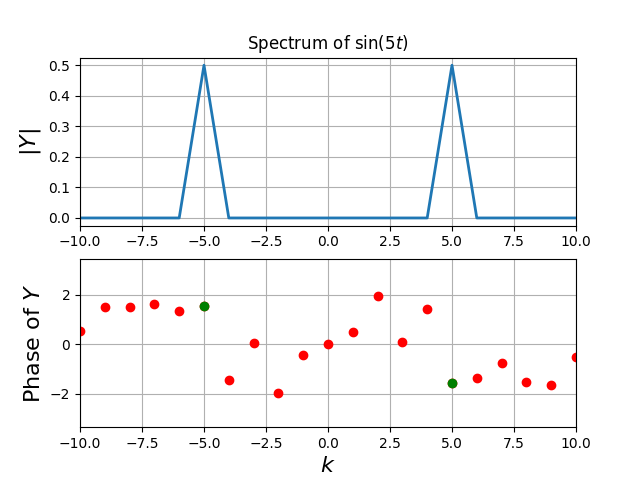
\includegraphics[scale=0.8]{ex2_f.png}
   	\label{fig:ex2_f}
   	\caption{Spectrum of $\sin(5t)$ - Trial 2}
\end{figure}
{
After the corrections we got the spectrum as we expected.
}


\subsection{EXAMPLE 3 - FFT of AM sinusoid - Trial 1} 
{
We try to take the FFT of an \textbf{Amplitude Modulated Sinusoid} of the form
$\left(1+0.1\cos\left(t\right)\right)\cos\left(10t\right)$
\\We can realise the peaks of CTFT and their amplitudes by noting that :
\[\cos(10t) + 0.1\cos(t)\cos(10t) = 1\cos(10t) + 0.05(\cos(11t) + \cos(9t))\]
\[\hspace{2cm} = 0.5( e^{10jt} + e^{-10jt} ) + 0.025( e^{9jt} + e^{11jt} + e^{-9jt} + e^{-11jt} )\]
}
\begin{minted}{python3}
t=linspace(0,2*pi,129);t=t[:-1]  #Low number of samples
y=(1+0.1*cos(t))*cos(10*t)  #AM with carrier at 10 and modulating freq of 1
Y=fftshift(fft(y))/128.0
w=linspace(-64,63,128)
figure()
subplot(2,1,1)
plot(w,abs(Y),lw=2)
xlim([-15,15])
ylabel(r"$|Y|$",size=16)
title(r"Spectrum of $\left(1+0.1\cos\left(t\right)\right)\cos\left(10t\right)$")
grid(True)
subplot(2,1,2)
plot(w,angle(Y),'ro',lw=2)
xlim([-15,15])
ylabel(r"Phase of $Y$",size=16)
xlabel(r"$\omega$",size=16)
grid(True)
savefig("eg3_i.png")
show()
\end{minted}

\begin{figure}[H]
   	\centering
   	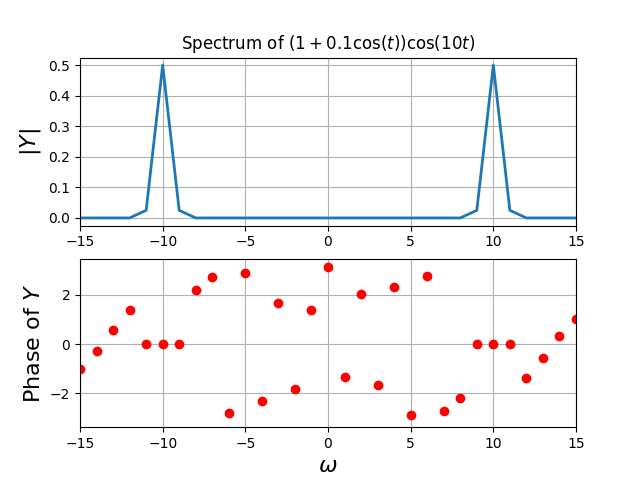
\includegraphics[scale=0.8]{eg3_i.png}
   	\label{fig:eg3_i}
   	\caption{Spectrum of $\left(1+0.1\cos\left(t\right)\right)\cos\left(10t\right)$ - Trial 1}
\end{figure}
{
We cant see three distinct peaks in the spectrum. This is because the \textbf{number of samples are not sufficient} to get the necessary information. This is known as \textbf{aliasing}.
}


\subsection{EXAMPLE 3 - FFT of AM sinusoid - Trial 2} 
{
We increase the number of samples and make sure aliasing does not occur.
}
\begin{minted}{python3}
t=linspace(-4*pi,4*pi,513);t=t[:-1]  #High number of samples, 
				  #hence tighter spectrum
y=(1+0.1*cos(t))*cos(10*t)
Y=fftshift(fft(y))/512.0
w=linspace(-64,64,513);w=w[:-1]
figure()
subplot(2,1,1)
plot(w,abs(Y),lw=2)
xlim([-15,15])
ylabel(r"$|Y|$",size=16)
title(r"Spectrum of $\left(1+0.1\cos\left(t\right)\right)\cos\left(10t\right)$")
grid(True)
subplot(2,1,2)
plot(w,angle(Y),'ro',lw=2)
xlim([-15,15])
ii=where(abs(Y)>1e-3)
plot(w[ii],angle(Y[ii]),'go',lw=2)
ylabel(r"Phase of $Y$",size=16)
xlabel(r"$\omega$",size=16)
grid(True)
savefig("eg3_f.png")
show()
\end{minted}
\begin{figure}[H]
   	\centering
   	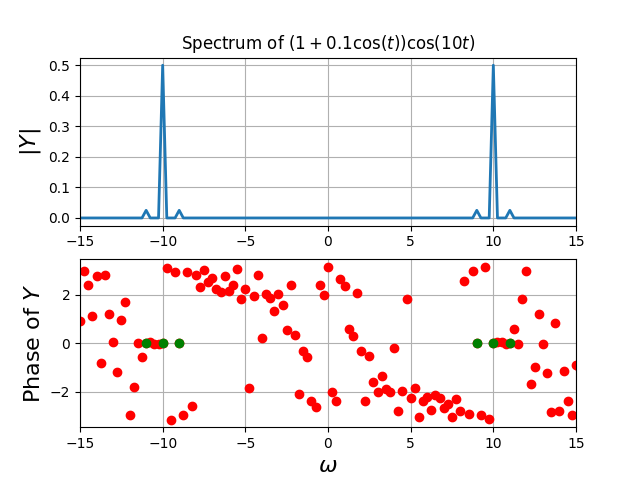
\includegraphics[scale=0.8]{eg3_f.png}
   	\label{fig:eg3_f}
   	\caption{Spectrum of $\left(1+0.1\cos\left(t\right)\right)\cos\left(10t\right)$ - Trial 2}
\end{figure}
{
Now, as we expected, we get \textbf{three peaks} at the carrier band and at frequencies above and below the carrier band at frequency difference equal to the \textbf{modulating frequency}.
Most of the energy is stored in the carrier band, as is evident from the amplitude of the peaks.
}


\subsection{DFT Utility Function}
{
We create a utility function DFT() to plot the DFT spectrum of different functions.
}
\begin{minted}{python3}
def DFT(y_fn,tim = (-4*pi,4*pi),N = 512,name = ''):
	''' Utility function for generating spectrum of given function.

	y_fn : function for which spectrum needs to be obtained
	tim : time interval of form (starting time,ending time) 
		where ending time has to be excluded
	N : number of samples in time domain
	name : Name of function for the spectrum
	'''
	st,end = tim

	t = linspace(st,end,N,endpoint = False)
	y = y_fn(t)
	Y = fftshift(fft(y))/float(N)
	w = linspace(-pi,pi,N,endpoint = False)
	w = w*(N/(end-st))
	fig, (ax1,ax2) = subplots(2,1)
	ii = where(abs(Y)>1e-3)
	ax1.plot(w,abs(Y),lw=1)
	ax1.set_xlim([-2*max(w[ii]),2*max(w[ii])])
	ax1.set_ylabel(r"$|Y|$",size=16)
	suptitle(f"Spectrum of {name}")
	ax1.grid(True)
	#Plotting only the phase of relevant points
	ax2.plot(w[ii],angle(Y[ii]),'go',lw=1)  
	ax2.grid(True)
	ax2.set_xlim([-2*max(w[ii]),2*max(w[ii])])
	ax2.set_ylabel(r"Phase of $Y$",size=16)
	ax2.set_xlabel(r"$\omega$",size=16)
	show()
\end{minted}


\subsection{QUESTION 2 - FFT for $sin^{3}(t)$ and $cos^{3}(t)$}
{
We use the defined DFT function to plot the DFT spectrum of the functions $sin^{3}(t)$ and $cos^{3}(t)$.
}
\begin{minted}{python3}
y1 = lambda t : (sin(t))**3
y2 = lambda t : (cos(t))**3

DFT(y1,(-4*pi,4*pi),256,r'$sin^{3}t$')
DFT(y2,(-2*pi,2*pi),256,r"$cos^{3}t$")
\end{minted}
\begin{figure}[H]
   	\centering
   	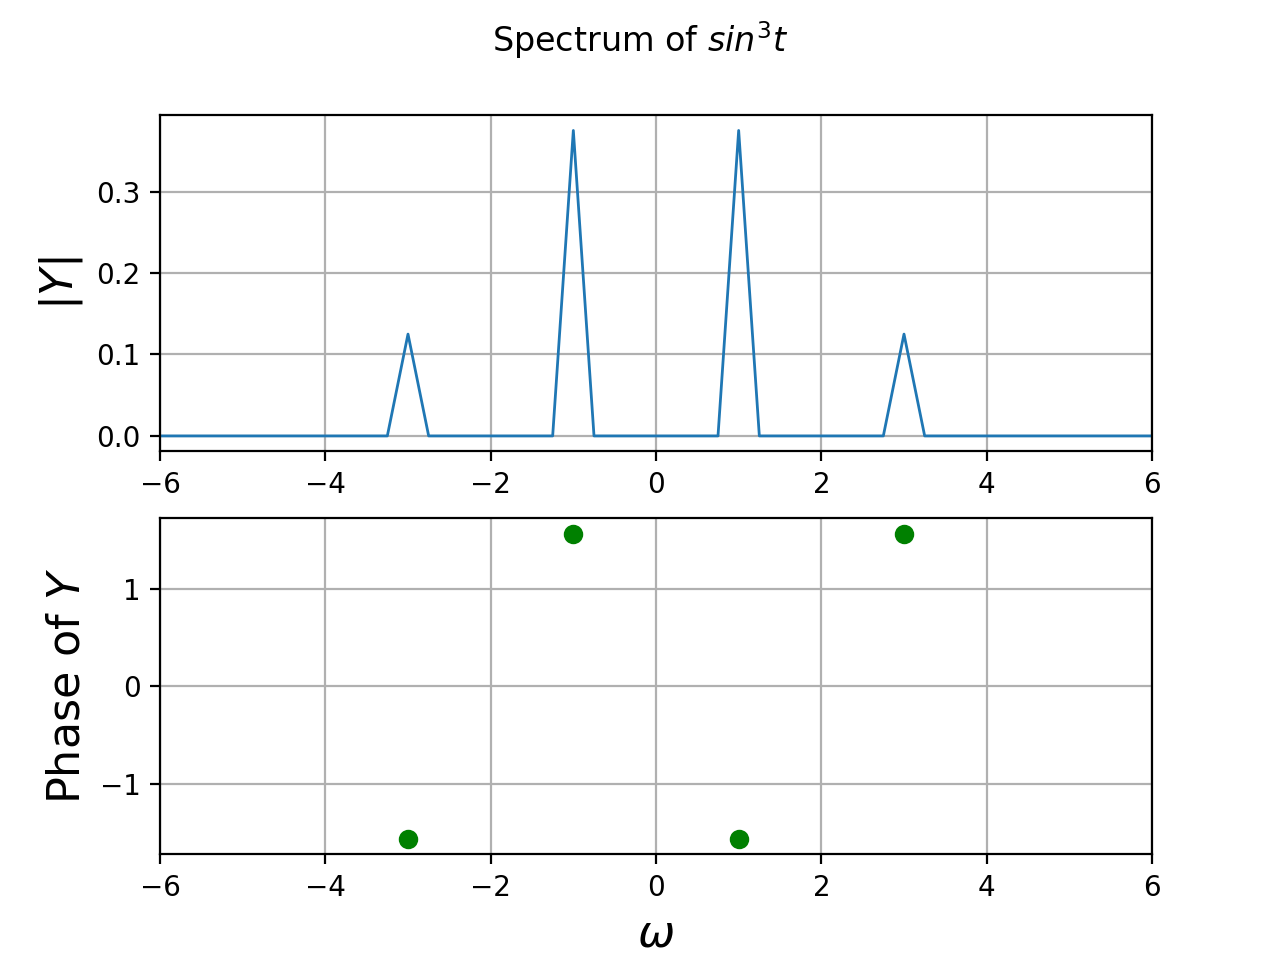
\includegraphics[scale=0.8]{qn2_sin3.png}
   	\label{fig:qn2_sin3}
   	\caption{Spectrum of $sin^{3}(t)$}
\end{figure}
{
The spectrum would have \textbf{4 peaks} as :
\[ \sin^3(t) =\frac{3\sin(t)-\sin(3t)}{4} \]
Thus we can also notice that the peaks corresponding to $\pm 1$ are thrice as big as the others.
}
\begin{figure}[H]
   	\centering
   	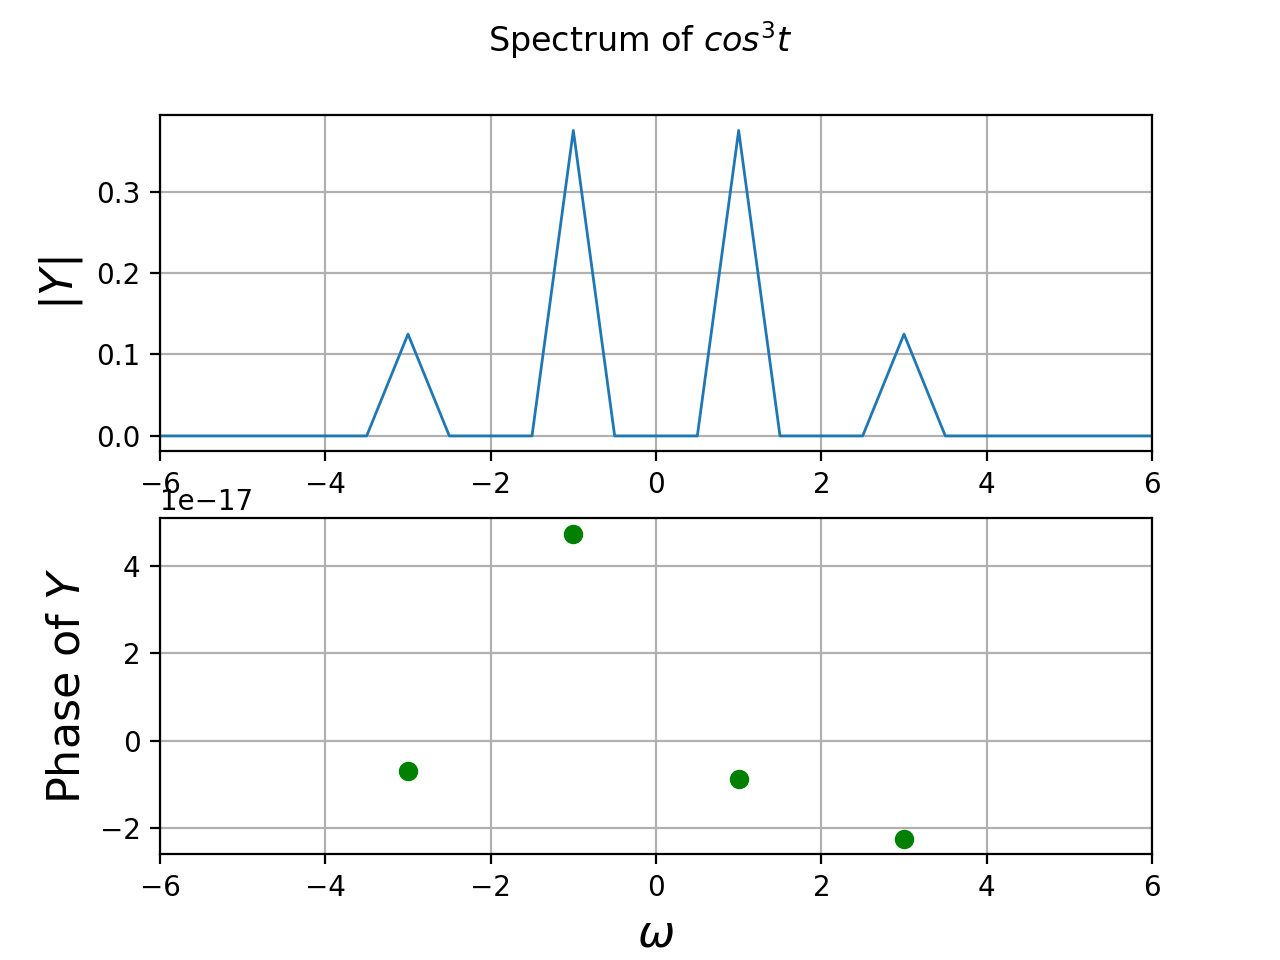
\includegraphics[scale=0.8]{qn2_cos3.png}
   	\label{fig:qn2_cos3}
   	\caption{Spectrum of $cos^{3}(t)$}
\end{figure}
{
Here :
\[ \cos^3(t) =\frac{ \cos(3t) +3\cos(t)}{4} \]
Hence there are \textbf{4 peaks} here too and the peaks corresponding to $\pm 1$ are thrice as big as the others.
}


\subsection{QUESTION 3 - FFT for FM sinusoid}
{
We plot the DFT spectrum of \textbf{frequency modulated sinusoid}.
$\cos(20t+5\cos(t))$
}
\begin{minted}{python3}
y3 = lambda t : cos(20*t+5*cos(t))

DFT(y3,(-4*pi,4*pi),2048,r"$cos(20t+5cos(t))$")
\end{minted}
\begin{figure}[H]
   	\centering
   	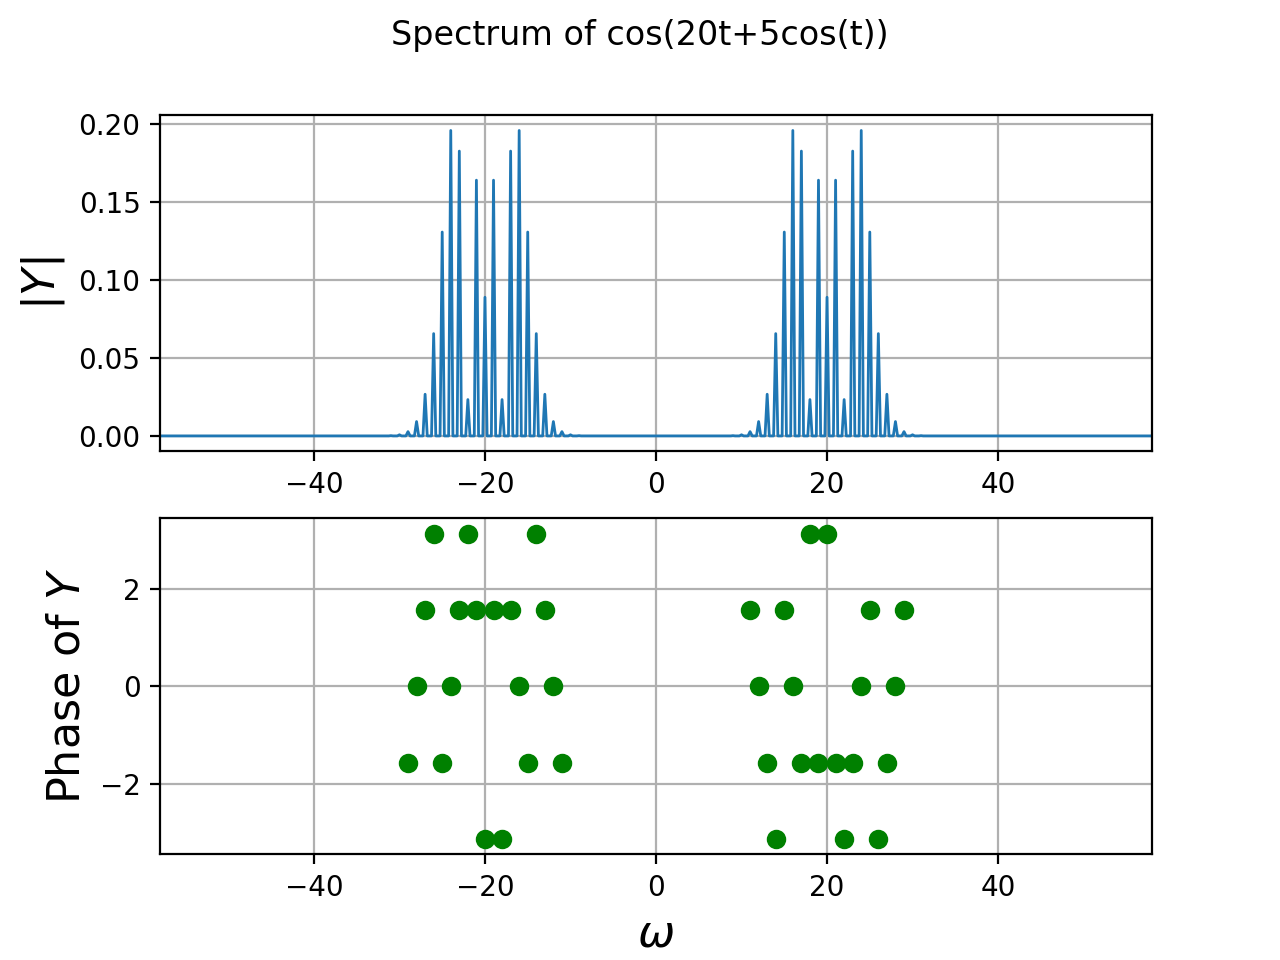
\includegraphics[scale=0.8]{qn2_FM.png}
   	\label{fig:qn3}
   	\caption{Spectrum of $\cos(20t+5\cos(t))$}
\end{figure}
{
A \textbf{lot of frequencies around the carrier band are present} and their energy is comparable to the carrier band.
}


\subsection{FFT for Gaussian}
{
We use the FFT to estimate the CTFT of the Gaussian distribution function
$e^{\frac{-t^2}{2}}$ which is not \textbf{Bandlimited} in frequency.
So we take a window of values of the Gaussian function and generate DFT from that as an approximate to the CTFT, since we know that the Gaussian function decays quickly on the left and the right. 
\\
The CTFT of the above aperiodic function is :
$\frac{e^{\frac{-\omega^2}{2}}}{\sqrt{2\pi}}$
}

\begin{minted}{python3}
def estCTFT(y_fn,org_fn,tim = (-4*pi,4*pi),N = 512,name = ''):
    ''' Utility function to plot DFT for Gaussian by taking a window of values
       and estimate how close the DFT is to the CTFT.

	y_fn : function for which spectrum needs to be obtained
	org_fn : the orginal CTFT function
	tim : time interval of form (starting time,ending time) 
		where ending time has to be excluded
	N : number of samples in time domain
	name : Name of function for the spectrum
	'''
    start,end = tim

    t = linspace(end,start,N,endpoint=False)
    y = y_fn(t)
    Y = fftshift(fft(ifftshift(y)))*(end-start)/(2*pi*N)  
    #Using ifftshift to remove phase issues

    w=linspace(-pi,pi,N,endpoint= False);
    w = w*(N/(end-start))
    
    ctft = org_fn(w)
    #Sum of absolute error between orginal CTFT and the DFT
    error = sum(abs(ctft-Y))
    print('Total absolute error between CTFT and DFT is :',error)
    
    fig, (ax1, ax2) = subplots(2, 1)
    ii = where(abs(Y) > 1e-3)
    suptitle("Spectrum of {}".format(name))
    #Plotting the orginal CTFT of Gaussian in the same plot
    ax1.plot(w,abs(ctft),'y-',label = 'CTFT')
    ax2.plot(w,angle(ctft),'yo',label = 'CTFT')

    ax1.plot(w,abs(Y),lw=1,label = 'DFT')
    ax1.set_xlim([-2*max(w[ii]),2*max(w[ii])])
    ax1.set_ylabel(r"$|Y|$",size=16)
    ax1.grid(True)
     #Plotting only the phase of relevant points
    ax2.plot(w[ii],angle(Y[ii]),'ro',label = 'DFT') 
    ax2.set_xlim([-2*max(w[ii]),2*max(w[ii])])  
    ax2.set_ylabel(r"Phase of $Y$",size=16)
    ax2.set_xlabel(r"$\omega$",size=16)
    ax2.grid(True)
    ax1.legend(loc = 'upper right')
    ax2.legend(loc = 'upper right')

    show()

y_gaussian = lambda t : exp(t**2/-2)
ctft_gaussian = lambda w : exp(-w**2/2)/sqrt(2*pi)

estCTFT(y_gaussian,ctft_gaussian,(-4*pi,4*pi),1024,r"$exp(-t^{2}/2)$")
\end{minted}
\begin{figure}[H]
   	\centering
   	
\includegraphics[scale=0.5]{qn4.png}
   	\label{fig:qn4}
   	\caption{Output of Total absolute error}
\end{figure}

\begin{figure}[H]
   	\centering
   	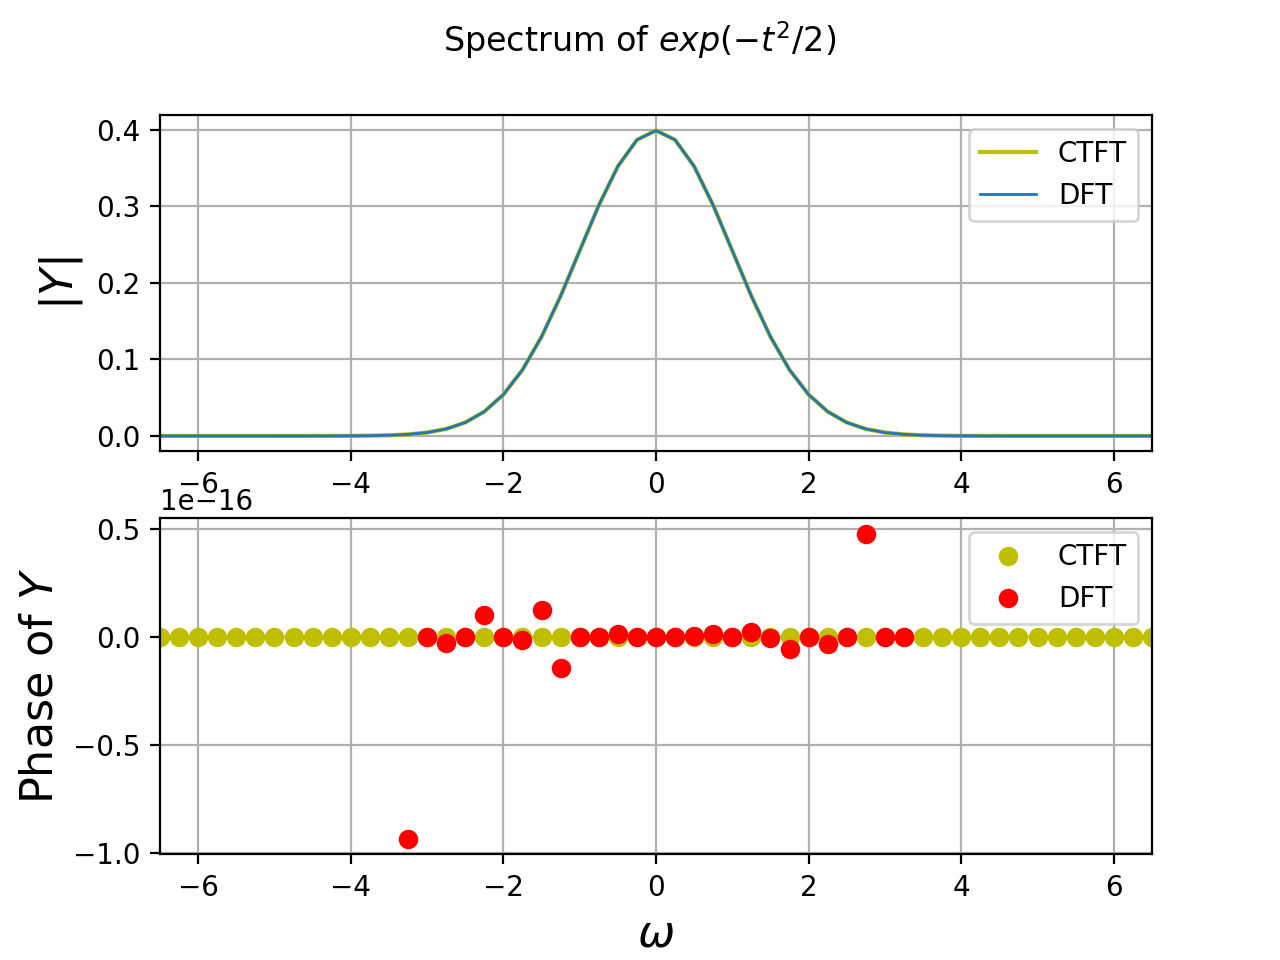
\includegraphics[scale=0.8]{gaussian.png}
   	\label{fig:gaussian}
   	\caption{Spectrum of $e^{\frac{-t^2}{2}}$}
\end{figure}

{
We can see that the total absolute error is very negligible (of the order $10^{-14}$) can be further reduced if necessary. However this error itself is almost zero to machine precision.
\\ifftshift() was used to remove certain phase issues with the time domain form of the Gaussian and make it ready for the fft().
\\Phase of DFT is basically zero (within numerical precision), indicating the CTFT of the Gaussian is real valued and positive for all $\omega$, just what the CTFT's phase plot predicts. In fact, the \textbf{CTFT of Gaussian is another gaussian function} as we can observe from the spectrum.
\\Thus it is clear that the Gaussian is the Eigenfunction of the Fourier Transform. 
}


\section{Conclusions}
\begin{itemize}
\item We analysed frequency domain spectra of various functions using numpy.fft
\item We understood how to correct the various problems that might occur while plotting the spectra.
\item We learnt to estimate CTFT of aperiodic bandlimited functions from DFT.
\end{itemize}

\end{document}